\documentclass[
  bibliography=totoc,     % Literatur im Inhaltsverzeichnis
  captions=tableheading,  % Tabellenüberschriften
  titlepage=firstiscover, % Titelseite ist Deckblatt
]{scrartcl}

% Paket float verbessern
\usepackage{scrhack}

% Warnung, falls nochmal kompiliert werden muss
\usepackage[aux]{rerunfilecheck}

% unverzichtbare Mathe-Befehle
\usepackage{amsmath}
% viele Mathe-Symbole
\usepackage{amssymb}
% Erweiterungen für amsmath
\usepackage{mathtools}

% Fonteinstellungen
\usepackage{fontspec}
% Latin Modern Fonts werden automatisch geladen
% Alternativ zum Beispiel:
%\setromanfont{Libertinus Serif}
%\setsansfont{Libertinus Sans}
%\setmonofont{Libertinus Mono}

% Wenn man andere Schriftarten gesetzt hat,
% sollte man das Seiten-Layout neu berechnen lassen
\recalctypearea{}

% deutsche Spracheinstellungen
\usepackage[ngerman]{babel}


\usepackage[
  math-style=ISO,    % ┐
  bold-style=ISO,    % │
  sans-style=italic, % │ ISO-Standard folgen
  nabla=upright,     % │
  partial=upright,   % │
  mathrm=sym,        % ┘
  warnings-off={           % ┐
    mathtools-colon,       % │ unnötige Warnungen ausschalten
    mathtools-overbracket, % │
  },                       % ┘
]{unicode-math}

% traditionelle Fonts für Mathematik
\setmathfont{Latin Modern Math}
% Alternativ zum Beispiel:
%\setmathfont{Libertinus Math}

\setmathfont{XITS Math}[range={scr, bfscr}]
\setmathfont{XITS Math}[range={cal, bfcal}, StylisticSet=1]

% Zahlen und Einheiten
\usepackage[
  locale=DE,                   % deutsche Einstellungen
  separate-uncertainty=true,   % immer Unsicherheit mit \pm
  per-mode=symbol-or-fraction, % / in inline math, fraction in display math
]{siunitx}

% chemische Formeln
\usepackage[
  version=4,
  math-greek=default, % ┐ mit unicode-math zusammenarbeiten
  text-greek=default, % ┘
]{mhchem}

% richtige Anführungszeichen
\usepackage[autostyle]{csquotes}

% schöne Brüche im Text
\usepackage{xfrac}

% Standardplatzierung für Floats einstellen
\usepackage{float}
\floatplacement{figure}{htbp}
\floatplacement{table}{htbp}

% Floats innerhalb einer Section halten
\usepackage[
  section, % Floats innerhalb der Section halten
  below,   % unterhalb der Section aber auf der selben Seite ist ok
]{placeins}

% Seite drehen für breite Tabellen: landscape Umgebung
\usepackage{pdflscape}

% Captions schöner machen.
\usepackage[
  labelfont=bf,        % Tabelle x: Abbildung y: ist jetzt fett
  font=small,          % Schrift etwas kleiner als Dokument
  width=0.9\textwidth, % maximale Breite einer Caption schmaler
]{caption}
% subfigure, subtable, subref
\usepackage{subcaption}

% Grafiken können eingebunden werden
\usepackage{graphicx}

% schöne Tabellen
\usepackage{tabularray}
\UseTblrLibrary{booktabs, siunitx}

% Verbesserungen am Schriftbild
\usepackage{microtype}

% Literaturverzeichnis
\usepackage[
  backend=biber,
]{biblatex}
% Quellendatenbank
\addbibresource{lit.bib}
\addbibresource{programme.bib}

% Hyperlinks im Dokument
\usepackage[
  german,
  unicode,        % Unicode in PDF-Attributen erlauben
  pdfusetitle,    % Titel, Autoren und Datum als PDF-Attribute
  pdfcreator={},  % ┐ PDF-Attribute säubern
  pdfproducer={}, % ┘
]{hyperref}
% erweiterte Bookmarks im PDF
\usepackage{bookmark}

% Trennung von Wörtern mit Strichen
\usepackage[shortcuts]{extdash}

\author{%
  Vincent Wirsdörfer\\%
  \href{mailto:vincent.wirsdoerfer@udo.edu}{authorA@udo.edu}%
  \and%
  Joris Daus\\%
  \href{mailto:joris.daus@udo.edu}{authorB@udo.edu}%
}
\publishers{TU Dortmund – Fakultät Physik}


\begin{document}
\section{Zielsetzung}


Das konkrete Ziel des folgend protokollierten Versuchs besteht darin den Elastizitätsmodul von Metallen verschiedener
Legierungen zu bestimmen. Ferner werden die empirisch ermittelten Werte mit der Literatur verglichen und somit deren
Aussagekraft bewertet.

\section{Theorie}
\label{sec:Theorie}
An einem Körper lässt sich genau dann eine Veränderung der Gestalt und des Volumens feststellen, wenn eine Kraft auf die
Oberfläche des Körpers einwirkt. Oftmals bezieht man diese Krafteinwirkung auf Flächeneinheiten, weswegen die physikalisch 
erhaltende Größe in diesem Fall die Spannung ist. Dabei muss jedoch zwischen zwei Spannungskomponenten unterschieden werden.
Einerseits gibt es den senkrecht zur Oberfläche stehenden Anteil der Spannung, welcher als \emph{Normalenspannung} $\sigma$
bezeichnet wird. Andererseit existiert zudem eine parallel zur Oberfläche stehender Anteil der Spannung. Dieser Anteil
heißt \emph{Tangentialspannung}. Ist nun die relative Änderung $\sfrac{\increment L}{L}$ einer linearen Körperdimension
hinreichend klein, so lässt sich ein proportionaler Zusammenhang zwischen dieser Änderung und der angreifenden Normalenspannung
$\sigma$ konstatieren. Präziser ausgedrückt wird dieser Zusammenhang durch das \emph{Hook'sche Gesetz}:

\begin{equation}
\label{eqn:Hook}
    \sigma = E\frac{\increment L}{L}
\end{equation}

\noindent Hierbei wird der Proportionalitätsfaktor dieser Gleichung als \emph{Elastizitätsmodul} beschrieben. Dieser 
repräsentiert eine wichtige Materialkonstante in der Werkstofftechnik.\\
Anhand von Gleichung \eqref{eqn:Hook} lässt sich nun vermuten, dass das Elastizitätsmodul durch eine bestimmte Messvorrichtung
und triviales Umstellen der Gleichung einfach zu errechnen ist. Aufgrund der Tatsache, dass solch eine Vorrichtung nicht immer
gewährleistet werden kann, wird sich bei diesem Versuch einer anderen Methodik, nämlich der \emph{Biegung} von elastischen
Stäben, bedient. Die theoretischen Grundgedanken hinter diesem Ansatz werden im Folgenden näher erläutert.

\subsection{Berechnung des E-Moduls bei einseitiger Einspannung des homogenen Stabes}

Wie bereits in der Theorie angeklungen, bedingt die Dehnung des Stabes nach Gleichung \eqref{eqn:Hook} eine Biegung des Körpers
was letztlich in einer Deformation resultiert. Dementsprechend muss eine Versuchsapperatur gefunden werden, welche es erlaubt,
die Durchbiegung $D(x)$ an verschiedenen Stellen $x$ zu messen. Eine solche Apperatur wird in Abbildung \ref{fig:Durchbiegung}
dargestellt.

\begin{figure}
    \centering
    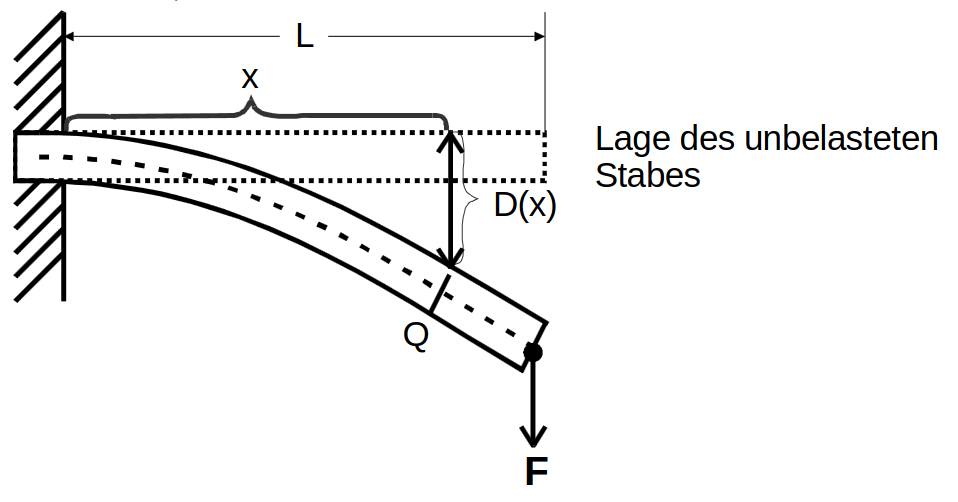
\includegraphics[height=5cm]{Durchbiegung.png}
    \caption{Durchbiegung eines elastischen Stabes bei einseitiger Aufhängung}
    \label{fig:Durchbiegung}
\end{figure}

%\noindent Es soll somit eine Menge von Wertepaaren $\{D(x)\x}$ bestimmt werden. Diese Messreihe wird dazu verwendet, den E-Modul
des Stabes zu berechnen, da die die Funktion $D(x)$ abhängig von $E$ ist. Die Gleichung muss somit nach $E$ umgesellt werden, um 
einen Wert für den Modul zu erhalten. Doch wie konkretisiert sich die Funktion $D(x)$ mathematisch genau?\\
An der Abbildung \ref{fig:Durchbiegung} ist zu erkennen, dass Kräftepaare auf den Stab einwirken, weswegen eine
\emph{Drehmomentgleichung} aufgestellt werden muss, um einen Ausdruck für $D(x)$ zu finden. Ferner zeigt die Abbildung, dass die Kraft $F$
auf den Querschnitt $Q$ ein Drehmoment $M_F$ bewirkt, welcher den Querschnitt aus seiner Ausgangslage verdreht. Dadurch werden,
die oberen Schichten des Stabes gedehnt und die unteren Schichten gestaucht. Elastische Eigenschaften des Stabes erzeugen jedoch
innere Normalenspannungen, welche dieser Biegung entgegenwirken. Zwischen der oberen und unteren Schicht existiert eine Fläche,
wo sich die Zugspannungen an der oberen Schicht und die Druckspannungen genau ausgleichen, weswegen hier in Summe keine Spannungen 
auftreten. Daher wird diese Fläche auch als \emph{neutrale Faser}\footnote{In Abb. \ref{fig:Durchbiegung} wird ihre Schnittline als gestrichelte Linie dargestellt.} bezeichnet.
Die entgegenwirkenden jedoch betragsmäßig äquivalenten Zug- und Druckspannungen erzeugen ein Drehmoment $M_\sigma$, welches sich wie folgt
berechnet lässt:

\begin{equation}
\label{eqn:Moments}
    M_\sigma = \int_Q y\sigma(y)\symup{d}q 
\end{equation}

\noindent Hierbei bezeichnet $y$ den Abstand des Flächenelements d$q$ zur neutralen Faser.\\
Wenn nun, wie in Abbildung \ref{fig:Durchbiegung} gezeigt, eine Kraft $F$, mit dem Hebelarm $L-x$ an einem Punkt des Stabes angreift, bedeutet dies
ein weiteres Drehmoment $M_F$ mit
\begin{equation}
\label{eqn:MomentF}
    M_F = F\left(L-x\right).
\end{equation}

\noindent Die Deformation stellt sich nun so sein, dass ein Gleichgewicht der Momente \eqref{eqn:Moments} und \eqref{eqn:MomentF} herrscht:

\begin{equation}
    \int_Q y\sigma(y)\symup{d}q =F\left(L-x\right)
\end{equation}



\end{document}